\section{Zielsetzung}
In diesem Versuch wird mit dem Photoeffekt der Zusammenhang zwischen der Maximalen Energei der emittierten Elektronen
und der Wellenlänge des Lichtes.
Zudem wird auch die Abhängigkeit des Elektronenstroms und der angelegten Spannung.

\section{Theorie}
\label{sec:Theorie}

Wird eine Metalloberfläche mit Licht bestrahlt, lösen sich Elektronen aus der Oberfläche.
Dies wird als Photoeffekt bezeichnet.

Das Licht wird in der Quantenelektrodynamik durch des Korpuskel- und Wellenmodell beschrieben, wobei diese Modelle als Grenzfälle betrachtet werden.
Bei der Ausbreitung von Licht, wird das Welllenmodell zur Erklärung verwendet.
Das Korpuskelmodell wird jedoch bei der Wechselwirkung von Licht mit Materie verwendet.
\subsection{Erklärung des Photoeffekts mithilfe des Korpuskelmodell}
Zur Untersuchung des Photoeffekts wird der Aufbau in Abbildung \ref{fig:phauf} dargestellt.
\begin{figure}
    \centering
    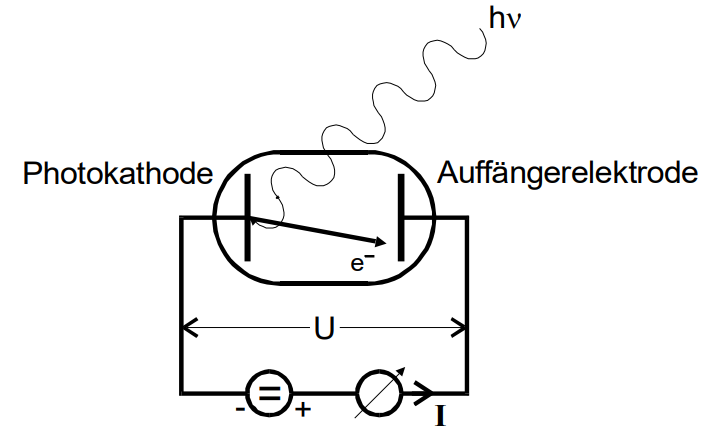
\includegraphics[scale=0.5]{content/PhoUnt.png}
    \caption{Aufbau zur Untersuchung des Photoeffekts.\cite{sample}}
    \label{fig:phauf}
\end{figure}
Die Photokathode in einer Vakuumröhre wird mit monochromatischem Licht bestrahlt.
Die Auffängerelektrode besitzt dabei ein positives Potential, wodurch die rausgelösten Elektronen sich zur Elektrode bewegen.
Das Experiment ergibt:
\begin{itemize}
    \item Die Anzahl der Photoelektronen pro Zeiteinheit ist proportional zur Lichtintesität. 
    \item Die Energie der Photoelektronen ist unabhängig zur Intensität des Lichts, allerding proportional zur Lichtfrequenz.
    \item Unterhalb einer Grensfrequenz, tritt der Photoeffekt nicht auf.
\end{itemize}   
Diese Ergebnisse lassen sich nicht nur mit dem Wellenmodell beschreiben.
Wenn das Licht als Welle angenommen wird, werden die Elektronen auf der Oberfläche zur Schwingung angeregt.
Die Rücktreibendekraft wird überwunden, wenn die Schwingungsamplitude groß genug ist.
Bei langwelligen Licht und hoher Intensität müsste der Photoeffekt auftreten.
Demnach würde bei einer bestimmten Frequenz Resonanz auftreten.
Dies steht jedoch im Widerspruch zu den Ergebnissen des Experiment.
Somit wird das Licht mit dem Korpuskelmodell beschrieben.
Es wird angnommen, dass dei Energie des Strahlungsfeld in Photonen oder Lichtquanten transporteirt werden.
Nach Einstein sind die Photonen mit den Planckschen Energiequanten identisch.
Das monochromatischen Licht der Frequenz $\nu$ besteht aus Photonen, welche die die Energie $E\nu$ besitzten.
Diese Energie wird auf ein Elektron auf der Oberfläche übertragen.
Die übertagene Energie teilt sich auf in die Austrittsarbeit $A_k$ die notwendig ist, um die Oberfläche zu verlassen und in die Kinetische Energie $E_\text{kin}$, mit der sich das rausgelöste Elektron weiter bewegen kann.
\begin{equation}
    h \nu = E_\text{kin} + A_k
\end{equation}
Wenn $h\nu < A_k$ gilt, kann der Photoeffekt nicht mehr auftreten.
Damit lässt sich das auftreten der Grenzfrequenz erklären  
Eine Photon kann höchstens ein Elektron auslösen.
Durch diese Annahmen, lassen sich die Ergebnisse des Experiments ohne Widersprüche erklären.


\subsection{Untersuchung des Photoeffekts}
In einer Photozelle lassen sich die Photoelektronen auslösen.
\begin{figure}
    \centering
    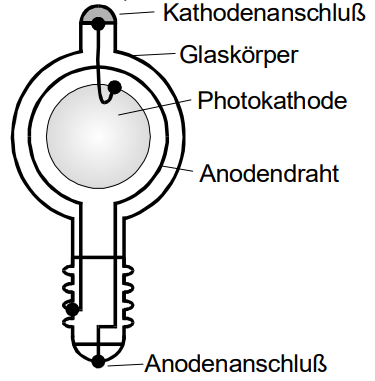
\includegraphics[scale=0.5]{content/Photozelle.png}
    \caption{Aufbau einer Photozelle.\cite{sample}}
    \label{fig:zelle}
\end{figure}
Die Innenseite der Photokathode besteht aus einem aufgedampften Metall-oder Legierungsschicht.
Diese kann mit Licht bestrahlt werden.
Die Anode besteht aus einem kreisförmigen Draht, welcher parallel zur Kathode angebracht ist.
Um die Energie der Photoelktronen zu messen, wird die sogenannte Gegenfeldmethode verwendet.
Dabei wird die Schaltung aus der Abbildung \ref{fig:gegenf} verwendet.
\begin{figure}
    \centering
    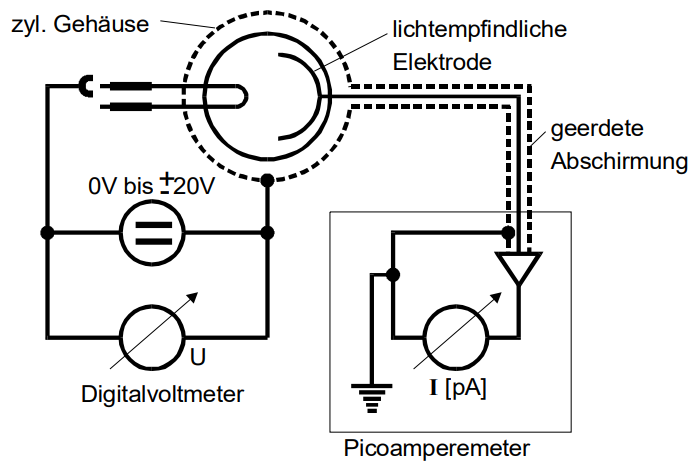
\includegraphics[scale=0.5]{content/Gegenfeld.png}
    \caption{Schaltbild der Messaperatur zur Gegenfeldmethode.\cite{sample}}
    \label{fig:gegenf}
\end{figure}
Wenn die kinetische Energie der Photoelktron größer als $e_0U_g$ ist, gelangen diese zur Anode.
Der Photostrom verschwindet, wenn 
\begin{equation}
    e_0 U_g = \frac{1}{2}m_0 v_\text{max}^2
\end{equation}
gilt.
Dabei beschreibt $U_g$ die angelegte Gegenspannung und $v_\text{max}$ die Geschwindigkeit des schnellsten Elektron beschreibt.
Die kinetische Energie der Photoelktronen sind unterschiedlich groß und hängen unteranderem von der Energie die die Elktronen schon im Festkörper hatte.
Die Fermi-Dirac-Statistik sagt über die Energie aus, dass diese zwischen 0 und der Fermi-Energie $\zeta$ liegt.
Der Verlauf des Photostroms wird in der Abbildung \ref{fig:verlauf} dargestellt.
\begin{figure}
    \centering
    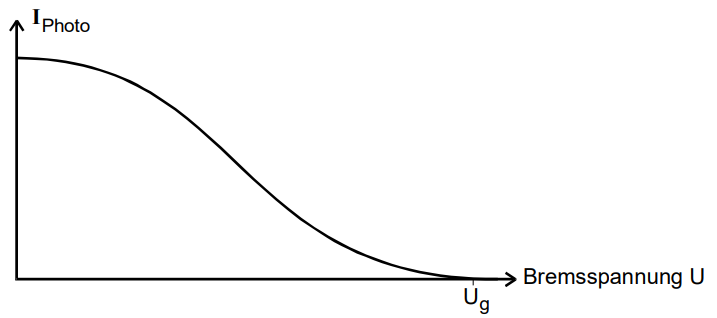
\includegraphics[scale=0.5]{content/VerlaufIU.png}
    \caption{Photostrom in Abhängigkeit der Gegenspannung.\cite{sample}}
    \label{fig:verlauf}
\end{figure}
Zwischen den Photostrom $I_\text{ph}$ und der Bremsspannung $U_g$ lässt sich ein parabolischer Zusammenhang
\begin{equation*}
    I_\text{ph} \sim U^2
\end{equation*}
Wenn die Austritsarbeit des Anodenmaterials $A_A$ zu groß ist, können die Elektronen die Anode nicht erreichen, da
diese das Gegenfeld nicht überwinden können.
Damit diese die Anode dennoch erreichen, wird eine Beschleungigungsspannung $U_b$ angelegt.
Ein Photostrom tritt dann auf, wenn
\begin{equation}
    h \nu + e_0 U_b \geq A_A
\end{equation}  
\cite{sample}
